%!TEX root = main.tex

\subsection{Building a Gold Standard Dataset for Evaluation}

In order to evaluate our approach we require a dataset of online information
seeking tasks which includes web clips from diverse web sources, with each
clip's topic labeled by human annotators. Unfortunately, we did not find any
existing datasets meeting these requirements, and thus developed our own. To do
so we found four questions that people asked on common Q\&A forums (e.g.,
StackOverflow, Yahoo! Answers) that seemed representative and covered a diverse
range of information needs. We then posted these questions to Amazon Mechanical
Turk (AMT), and asked crowdworkers to provide five webpages that best answered
the question (Table \ref{tab:datasets}). We then posted the most highly cited
sources across crowdworkers to AMT again, and asked workers to highlight clips
in the sources that help answer the question via an interface similar to that
described in \cite{kittur2013costs}.  The datasets collected consists of 75 to
100 clips, extracted from 7 to 19 webpages using 12 to 19 crowdworkers. A
preliminary study suggested that these were sufficient to provide comprehensive
information for answering these questions, though increasing the number of
sources may provide other benefits such as making users more confident in the
information. 

Two human judges clustered each of the four datasets. No discussion on
clustering strategies nor pre-defined categories were made prior to the
labeling process.  To measure inter-annotator agreement in a way that accounts for
both the number of clusters and their matches, we use the symmetric Normalized
Mutual Information metric (described in more detail below) as it better deals
with issues such as differing cluster sizes, large numbers of clusters, and
computational complexity than the clustering adaptation ($K_{max}$) of the
commonly used Cohen's kappa \cite{manning2008introduction,reilly2005rapid}. 

The results are shown in Table~\ref{tab:results}. The datasets
for ``\emph{How do I unclog my bathtub drain?}'', ``\emph{How do I get my
	tomato plants to produce more tomatoes?}'' and ``\emph{What are the best day trips possible from Barcelona?}'' have high agreement between the
two annotators of around 0.7 to 0.75 of NMI scores.  The clips were grouped by the different \emph{tools},
\emph{strategies}, \emph{environmental factors} and \emph{destinations} described in the clips. For
the ``\emph{What does a planet need to support life?}'' dataset, the agreement
is significantly lower. By examining the data, we found two reasons.  First,
there is a lot of uncertainty in the topic, because not even the science
community has a clear idea of the answer; for example, some clips even discussed whether
the definition of life should be exclusively carbon based. Second, there are a
lot of interconnected and correlated factors. For example, the \emph{distance
	to its star} determines whether a planet is in the \emph{habitable zone} of
a solar system, which effects the \emph{temperature} of the planet and whether
it potentially contains \emph{liquid water}. Even though we think both
independently created labels are valid ways of organizing this dataset, it also
suggests that a flat, or even a tree, structure might not be sufficient to
accurately organize this dataset. We return to this interesting challenge in
the discussion section. The final gold-standard labels were created by the two
judges labeling the entire datasets together for the second time, and reaching
agreement through discussion.

\subsection{Experimental Conditions}
We had two goals in our evaluation.  The first was external validation:
comparing our clustering approach to common existing machine learning
approaches. We compare our approach to four baselines that are commonly used in
the clustering literature.  Latent Dirichlet Allocation (LDA)
\cite{blei2003latent} is a widely used generative model under which each
document is generated with multiple topics, and each topic is a probability
distribution of words.  It is difficult for topic models to perform well for
collections of short text, since LDA relies on counting words in the documents
as probability distributions to discover topics. In our work, we focused on
organizing small web clips that typically have a single topic, contradicting
the assumptions of the LDA generative model. On the other hand, latent semantic
analysis (LSA) \cite{deerwester1990indexing} seemed more suitable for our goals.
It reduces word vector dimensions by grouping words together to form concept
dimensions based on their occurrence in similar documents. We also compared our
approach to two other commonly used baseline approaches to computing similarity
for clustering, including simple cosine similarity based on human-identified
keyword vectors, and TF-IDF weighted cosine similarity
\cite{manning2008introduction,Jones72astatistical}. The former tests served as
a control for whether our approach has value beyond the human identification of
relevant keywords, while the latter automated the keyword selection based on
term and document frequencies. The baseline systems required different
parameters as additional inputs (i.e., stopping threshold, number of topics,
number of dimensions, priors, ..., etc.).  Some of these parameters can be
time-consuming to fine-tune \cite{chuang2012termite}.  Therefore, for each
question, we iterated on different parameter combinations for each of the
baseline systems, and reported the best score to compare with our method.


The second goal was internal examination: evaluating the assumptions of our
approach and characterizing its performance under varying conditions. One way we
do so is to report the performance of the approach under varying numbers of crowd workers,
which can help to characterize the cost/benefit tradeoffs in involving human judgments
in the process. Another way we do so is to compare the performance of a two-phase process
with a one-phase control. Specifically, in addition to running a combined Phase A and Phase B condition, we run a Phase A-only condition in which we add additional crowd workers equal
to the number that would have worked on Phase B.  We call these two conditions System AB and System A, respectively.

These different evaluation conditions are summarized below:

\begin{itemize}
	\item \emph{System A}. The partial system with twenty crowdworkers and
		Phase A only.
	\item \emph{System AB}. The complete system with ten crowdworkers for each
		Phase A and Phase B.
	\item \emph{TF-IDF}. TF-IDF weighted cosine similarity is used as the
		similarity function for hierarchical clustering of the input dataset.
		No human-computation was employed in this baseline system.
	\item \emph{Worker keywords}. Cosine similarity based on worker-highlighted keywords from Phase A are used as the
		similarity function for hierarchical clustering of the input dataset. This condition aims to test the value of the approach beyond the human identification of keywords.
	\item \emph{LSA}. The LSA model is used as the similarity function for
		hierarchical clustering.  No human-computation was employed for this
		baseline system.
	\item \emph{LDA}. The LDA topic model is used as the similarity function
		for hierarchical clustering.  No human-computation was employed for
		this baseline system.
\end{itemize}

\subsection{Evaluation Metric: Normalized Mutual Information}

Unlike evaluating a classification task, which would typically be based on
the precision and recall rate of pre-defined classes, evaluating clusters is not as
straightforward. For example, the output of the system and the gold standard
can have different number of clusters. They can either be many-to-one mappings
(mapping multiple fine-grained clusters to a more abstract cluster), or
clusters created based on different concepts. It is also not as informative to
use precision and recall to evaluate clustering results. For example, the
purity metric computes the average precision of all clusters in the system
output, however, maximum purity can be easily achieved if each clip is its own
cluster. Instead, we use the Normalized Mutual Information from Information
Theory and Information Retrieval to evaluate the difference between system
output and the gold-standard clusters \cite{manning2008introduction}. The NMI
metric is a symmetric measurement sensitive to both the number of clusters, and
the precision of each cluster.  Specifically, it compares all possible
cluster mappings to calculate the mutual information, and divide it by the mean
entropy of the two sets of clusters so that results across different datasets
are comparable, and unbiased by the innate complexity of different
questions.

The normalized mutual information is defined as:

\begin{equation}
NMI(\Omega, C) = \frac{I(\Omega, C)}{0.5 * [H(\Omega) + H(C)]}
\end{equation}

where $\Omega$ is the output clusters and $C$ is the gold-standard clusters.
The mutual information $I$ between the two sets of clusters is defined as:


\begin{equation}
	\begin{split}
I(\Omega, C) & = \sum_k \sum_j P(\omega_k \cap c_j) log \frac{P(\omega_k \cap c_j)}{P(\omega_k)P(c_j)} \\
             & = \sum_k \sum_j \frac{|\omega_k \cap c_j|}{N} log \frac{N|\omega_k \cap c_j|}{|\omega_k||c_j|}
	 \end{split}
 \end{equation}

where $\omega_k$ and $c_j$ denotes each of the clusters in $\Omega$ and $C$,
respectively.  Finally, the entropy $H$ of a single set of clusters is defined
as:

\begin{equation}
	\begin{split}
H(\Omega) & = - \sum_k P(\omega_k) log P(\omega_k) \\
          & = - \sum_k \frac{|\omega_k|}{N} log \frac{|\omega_k|}{N}
	\end{split}
\end{equation}


\subsection{Evaluation Results}

As shown in Table \ref{tab:results}, the full System AB (with both Phase A and
Phase B) performed the best in all four questions with NMI scores
higher than System A and all baseline comparisons. For some questions System AB
performed much better than all baselines (e.g., unclog drain, grow tomatoes)
while for one question (habitable planet) it was essentially the same performance as LSA.
However, for the latter question all of the approaches had significant trouble,
including low agreement between human annotators. These results suggest that using crowdworkers to refine outputs from a machine learning model can be an effective strategy. Of the four
baseline systems, LSA performed the best.  Worker-identified keywords consistantly outperformed TF-IDF, showing that the crowdworkers are extracting keywords in Phase A that are salient for identifying clusters each dataset. However, it did not outperform the
full System AB, suggesting that there is significant value in the second phase of
classifying low-confidence items.

In Figure \ref{fig:numberOfTurkers}, we show the performance of System A and
System AB employing different number of crowdworkers.  Initially, increasing the
number of training data in Phase A showed significant performance improvement.
After gathering training data from around ten crowdworkers, the amount of performance
gain from hiring additional crowdworkers decreases notable. However, the
results also showed that performance improved significantly even with only a few crowdworkers in Phase B to refine the clusters from Phase A. Finally,
with twenty crowdworkers, the system with 10 crowdworkers in each Phase
consistently outperforms having all 20 crowdworkers in Phase A.

These results show that the complete System AB can produce clusters with NMI
difference to the gold-standard clusters close to the NMI difference between
the two annotators. Although this does not necessarily mean the system produces
expert results, it suggests that the output is comparable to that produced
by the judges who had a global view of the datasets and multiple rounds of reading,
labeling, and discussing them.



\begin{figure}[!t]
	\centering
	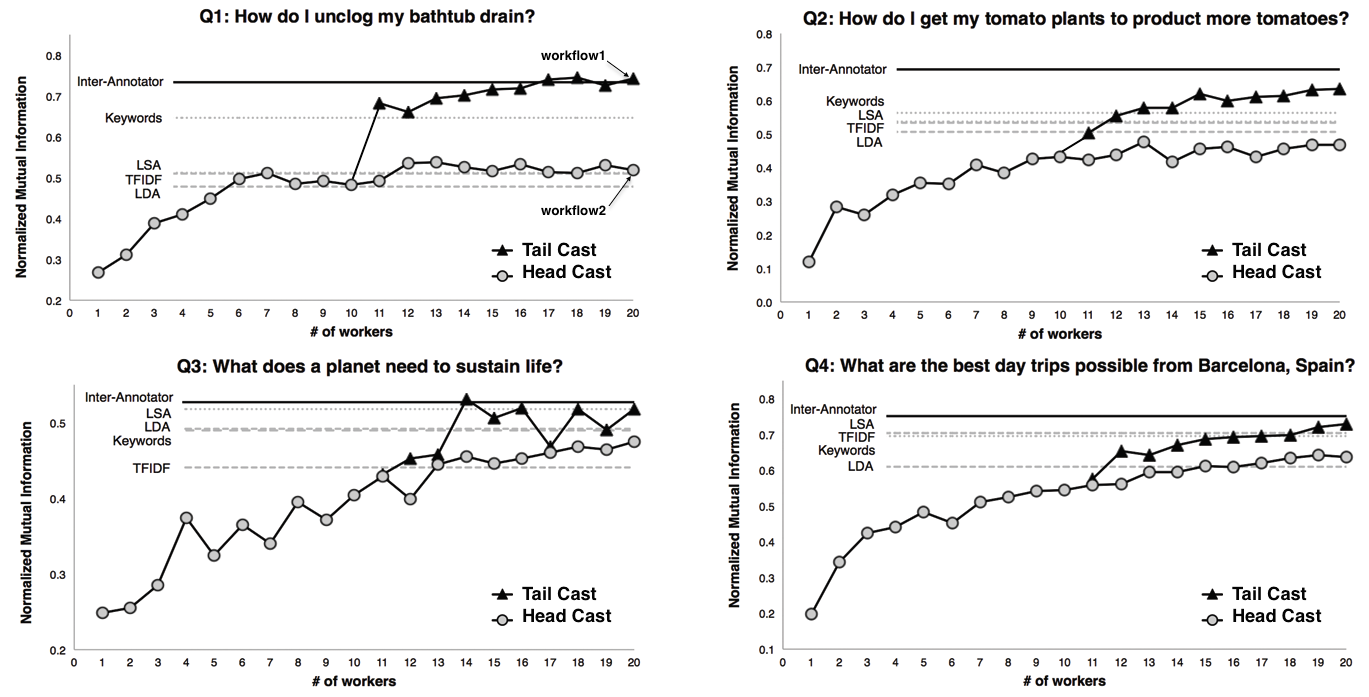
\includegraphics[width=1\columnwidth]{images/numberOfTurkers.png}
	\caption{Performance comparison of using diferent number of crowdworkers in Phase A and Phase B.}
	\label{fig:numberOfTurkers}
\end{figure}

\begin{table}
  \centering
% question, number of sources, number of clips, number of turkers
  \begin{tabular}{ c r r r r r r r }
    \hline
	Questions &
	Inter-annotator &
	System A &
	System AB &
	TF-IDF &
	Keywords &
	LSA &
	LDA \\
    \hline
	% 102
	\textbf{Q1} & .7335 & .5190 & \textbf{.7415} & .5099 & .6465 & .5118 & .4780 \\

	% 115 - 2
	\textbf{Q2} & .6928 & .4691 & \textbf{.6347} & .5339 & .5621 & .5373 & .5063 \\

	% 96
	\textbf{Q3} & .4768 & .4247 & \textbf{.4680} & .3901 & .4397 & .4674 & .4417 \\

	% 116
	\textbf{Q4} & .7499 & .6333 & \textbf{.7272} & .6728 & .6762 & .7038 & .6028 \\

%	% 137 carbon footprint
%	\textbf{Q5} & .6303 & .? & ? & .? & .? & .? & .? \\
%
%	% 139
%	\textbf{Q6} & .? & .? & ? & .? & .? & .? & .? \\
    \hline
  \end{tabular}
  \caption{Evaluation results}
  \label{tab:results}
\end{table}




% \subsection{Crowdworkers}

% The crowdworkers employed to test the proposed method are recruited from Amazon
% Mechanical Turk. With a total of 65 unique workers participated in the
% experiments, 56 of them have IP addresses origin in the United States, 6 of
% them from India, and 3 from other regions. From self-reporting, 40 workers are
% males and 25 workers are females, 8 workers are between the age of 18 to 24, 40
% workers are between the age of 25 to 34, 15 workers are between the age of 35
% to 44, and the rest in other ranges or chose not to report. Each worker is paid
% 1.00 USD for completing one of the two HITs. Therefore, the costs for both
% System A and System AB is 20.00 USD.

% \begin{table*}
%   \centering
% % question, number of sources, number of clips, number of turkers
%   \begin{tabular}{ c l l l l l }
%     \hline
% 	\tabhead{} &
% 	\tabhead{Phase A Mean} &
% 	\tabhead{Phase A Std. Dev} &
% 	\tabhead{Phase B Mean} &
% 	\tabhead{Phase B Std. Dev} &
% 	\tabhead{ANOVA P-Value} \\
%     \hline

% 	Interface & 4.2270 & 0.6477 & 3.710 & 0.783 & $\sim$ 0.000 \\ 
% 	Instructions & 4.0286 & 0.9592 & 3.786 & 1.001 & $\sim$ 0.156 \\
% 	Difficulty & 3.5099 & 1.0255 & 3.119 & 1.109 & $\sim$ 0.033 \\

%     \hline

%   \end{tabular}
%   \caption{Survey feedback from the crowdworkers.}
%   \label{tab:feedback}
% \end{table*}


% \subsection{Survey feedback from Crowdworkers}
% Upon completion of each HIT, we asked each unique worker to rate the task
% description, interface design, and overall difficulty of the HITs by filling
% out a survey form. We used a 5-point Likert scale, ranging from ``Strongly
% Agree'' (5) to ``Strongly Disagree'' (1) in order to gauge their opinions
% regarding the different features of the HIT. As shown in Table \ref{tab:feedback}, workers
% thought that the interface from Phase A was easier to utilize than interface
% for Phase B (p-value $\sim$ 0.000), with their average response being that they
% agreed that Phase A's interface was easy to use, while Phase B's interface
% was acceptable. There was not a significant difference between their responses
% regarding the instructions, agreeing that for both phases the instructions were
% easy to understand and follow. Finally, workers thought that Phase A was easier
% than Phase B (p-value $\sim$ 0.033), with neither task being considered to be
% particularly easy to complete. 

% We also allowed the Crowdworkers to comment on the HITs, and many of them find
% the clustering process interesting and enjoyable, leaving comments such as
% ``This was an interesting hit. I enjoyed it.'', ``very interesting to name each
% clusters'', and ``This was an interesting study and I actually learned a new
% tip to try and clear a clogged drain.'' 


%\begin{table*}
%  \centering
%% question, number of sources, number of clips, number of turkers
%  \begin{tabular}{ l r r r r r }
%    \hline
%	\tabhead{Questions} &
%	\tabhead{strongly agree} &
%	\tabhead{agree} &
%	\tabhead{neither...} &
%	\tabhead{disagree} &
%	\tabhead{strongly disagree} \\
%    \hline
%    \multicolumn{6}{c}{\tabhead{Phase A}} \\
%    \hline
%	% 54
%	\emph{I find this task easy to complete} & 11\% & 46\% & 31\% & 11\% & 0\% \\
%  
%	% 53
%	\emph{The instructions clearly explain the task} & 34\% & 55\% & 8\% & 4\% & 0\% \\
% 
%	% 54
%	\emph{The user interface is easy to learn and use} & 40\% & 56\% & 4\% & 0\% & 0\% \\
%    \hline
%    \multicolumn{6}{c}{\tabhead{Phase B}} \\
%    \hline
%	% 54
%	\emph{I find this task easy to complete} & 9\% & 45\% & 9\% & 36\% & 0\% \\
%
%	% 53
%	\emph{The instructions clearly explain the task} & 18\% & 55\% & 11\% & 11\% & 11\% \\
%
%	% 54
%	\emph{The user interface is easy to learn and use} & 27\% & 55\% & 11\% & 11\% & 0\% \\
%    \hline
%
%  \end{tabular}
%  \caption{Survey feedback from the crowdworkers.}
%  \label{tab:feedback}
%\end{table*}

